\documentclass[10pt, twocolumn]{article}
\usepackage[margin=1in]{geometry}
\usepackage{graphicx}
\usepackage{subcaption}
\usepackage{float}

\title{Deep Reinforcement Learning for Atari Games}
\author{Garnet Liu \and Vikram Saraph \and Birol Senturk}

\begin{document}
\maketitle

\begin{abstract}

Model free agents can perform very well on certain tasks, but they tend to  have trouble when a greedy approach is not optimal, or precise planning is required for success.
"Imagination-Augmented Agents for Deep Reinforcement Learning" 

\end{abstract}

\section{Introduction}

In recent years, deep learning techniques have been successfully adapted and applied to problems
in reinforcement learning. In this project, we survey and evaluate one such technique, called \emph{imagination augmented agents}, or \emph{I2A}. This technique was initially developed and published by Weber \emph{et. al.} at DeepMind \cite{I2A}. In their original
work, the authors describe the novel I2A as one that combines aspects of \emph{model-free} learning, in which an agent makes decisions based only on its state and reward observations, with \emph{model-based} learning, where the agent attempts to learn
about its environment in addition to a policy. In their work, the model-free agent is augmented with a model-based \emph{imagination engine}, which makes predictions about future trajectories of the agent from its current state.

While model-free agents have seemingly more flexible architectures, in practice they do not generalize very well to different tasks,
since they can exhibit poor performance. Incorporating model-based aspects allows one to provide additional fine-tuning to the network's architecture in a way that is specific of the 
agent's environment. Indeed, the authors of the original paper demonstrate a significant improvement in the agent when adding 
imagination to a standard model-free agent. They apply I2A to two different 2D games: MiniPacman, which is a simplified version of 
PacMan, and Sokoban, in which the agent must push blocks onto designated targets to solve each level.

In this work, we focus on applying I2A to Pong. First we provide a general background on the I2A architecture, in addition
to the gaming environment we use to simulate Pong. Then we describe our implementation and design decisions we made when applying I2A to Pong, and conclude with results from our implementation and discussion on issues and potential future work.

\section{Related Work}
As with many machine learning models, the original work on the Actor-Critic algorithm long proceeded the recent explosion deep learning literature \cite{A2C}. Asynchronous Actor-Critic, or A3C \cite{A3C}, further builds upon A2C by parallelizing the work performed by the original algorithm in an asynchronous manner. A3C is thus capable of better exploiting modern multicore architectures, and is the backbone of the model-free component of I2A.

We implement I2A in TensorFlow. While there does not appear to be an official implementation of I2A by DeepMind, we referred to a PyTorch implementation found on GitHub \cite{} as a guideline for our implementation.

\section{Background}

In this section, we provide a high-level overview of the I2A architecture as described in the original work. See the Methodology section for more specifics on how we applied this architecture to our Pong use case.

I2A unifies a model-free 
architecture and a model-based one. The model-based component of I2A is also referred to as the imagination engine, and consists of a 
sequence of \emph{imagination cores} that collectively generate a predicted future trajectory. Each imagination core makes use of a pre-trained policy network and an environment model. The policy network predicts the best action to take given an input state. The environment model takes an input state and the action returned by the policy network, and predicts the next state from taking the action. The predicted next state is fed from one imagination core to the subsequent one, so in this way, the output of the imagination cores is a sequence of predicted states (or trajectory). This trajectory provides additional context when learning a policy; together, the model-free policy and the imagine engine are combined to train a unified policy.

\section{Game Environment}
The Arcade Learning Environment (ALE) is used to simulate playing Atari games, so we use this to play and interact with
Pong. ALE has been integrated into OpenAI Gym \cite{openai}, which provides a standardized interface for taking actions
and retrieving the resulting new state, reward, etc. The game's state is simply the RGB image of a frame at a given point in time,
though many games have an alternative API that returns the RAM's state instead.

Before image data is fed into any part of the network, it is normalized in a way that is more convenient for training.
In particular, the top the image is removed, since it is only used to display the players' scores, pixels of which are
unlikely to be useful features for learning to play the game. In addition, the top and bottom border color is changed from
white to black, since it is the same color as the ball. The idea is to help the network distinguish between the two types of pixels.
See Figure \ref{screenshots} below for a frame and its normalization.

\begin{figure}[h]
\centering
\begin{subfigure}[b]{.2\textwidth}
  \centering
  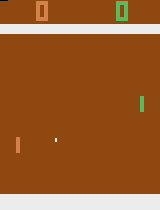
\includegraphics[scale=0.5]{unnormalized}
  \caption{Original image}
  \label{fig:unnormalized}
\end{subfigure} 
\begin{subfigure}[b]{.2\textwidth}
  \centering
  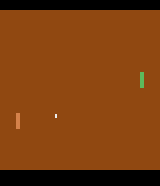
\includegraphics[scale=0.5]{normalized}
  \caption{After normalization}
  \label{fig:normalized}
\end{subfigure} \hfill
\caption{Pong screenshots before and after normalization.}
\label{screenshots}
\end{figure}

The OpenAI Gym API provides rewards and states, so we work with this data when training our model.
Actions are taken with the \verb|step| function.

\section{Methodology}

The model is trained in three phases. First, a model-free agent is trained by playing the game and using
A2C to learn. Once the model-free agent is trained, its policy is used to train the environment model.
The environment is trained by using the model-free agent's policy to play the game; by doing so it learns the
environment. In the following, we outline the structure of our TensorFlow program.

\begin{figure*}
\centering
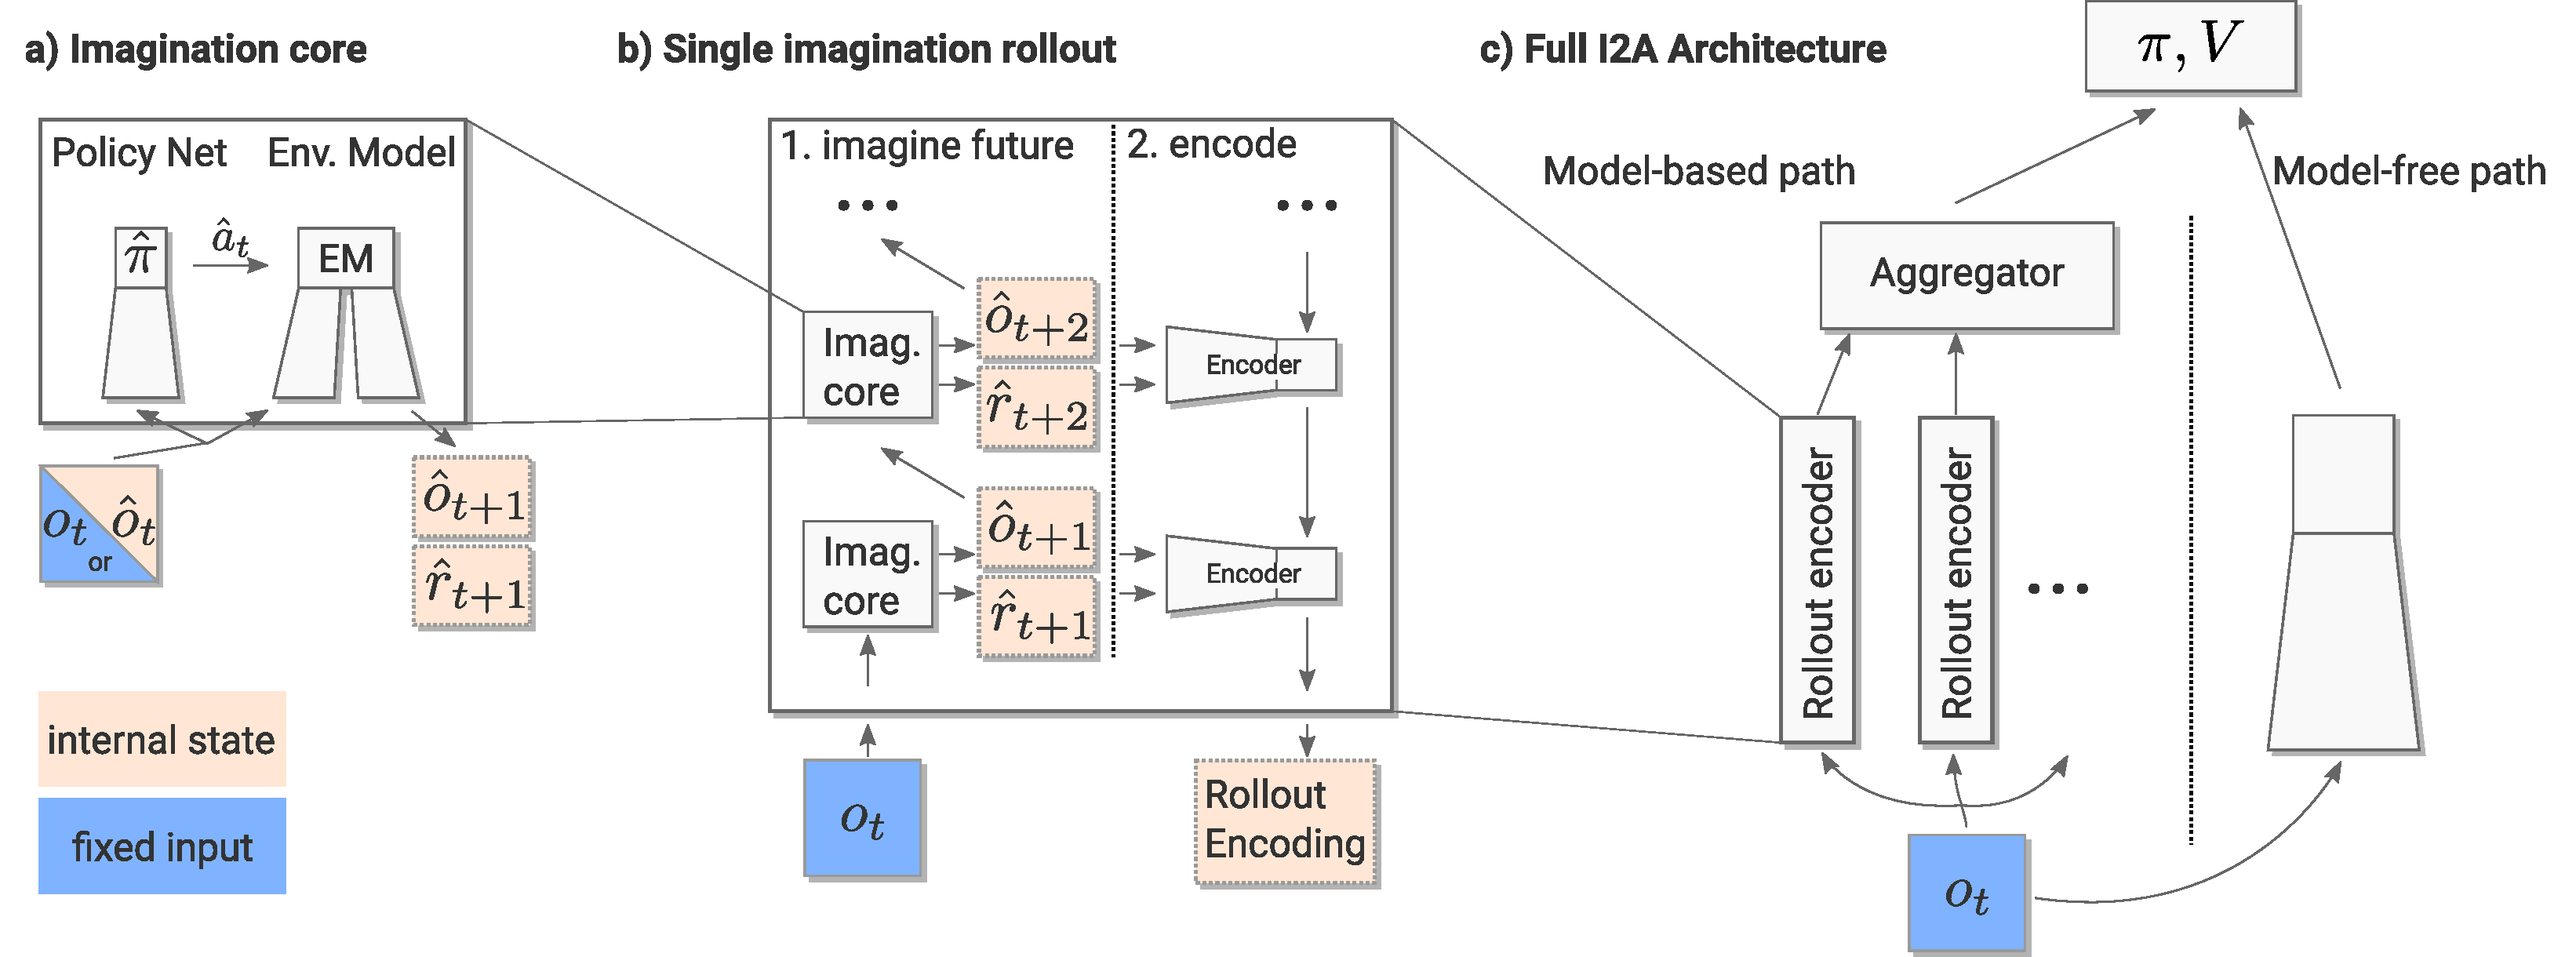
\includegraphics[scale=0.3]{i2a}
\caption{I2A architecture}
\end{figure*}

\subsection{Model-free agent}
ALE provides two different state spaces for playing Atari games, RAM content and the rendered pixels. We decided to use the pixel output, and stacked the current frame on top of the previous one to give the network some directional information which would in principle make our model-free agent easier to train.

While the original paper used an A3C (Asynchronous Actor-Critic) architecture as its model-free policy network, we decided to use the simpler A2C architecture.
The main difference is that A3C uses independent workers to update a shared policy network asynchronously, while A2C updates its weights sequentially.
A2C networks are harder to train, but easier to implement.
A2C contains an Actor that takes in an observation and produces a probability distribution over possible actions, and a Critic that also takes in an observation and assigns a numeric value to the observation which is then used to determine how advantageous a certain action is given the observed state.
While these can be two separate networks, we decided to use one network with two heads instead.
Input first goes through a stack of three convolutional layers and a fully connected layer that forms the trunk.
The output of this network is fed into separate Actor and Critic components which are two fully-connected layers and one output layer each.

\subsection{Environment model}

The computation graph of the environment model's network begins by using the policy described in the
previous section to take an action. Given an action and current state, recall that the environment model
predicts the next state and reward obtained. In general, the environment model's architecture should be
designed for the specific game in mind; however, for this project we used a modified version of the
MiniPacman environment model.

\begin{figure}[H]
\centering
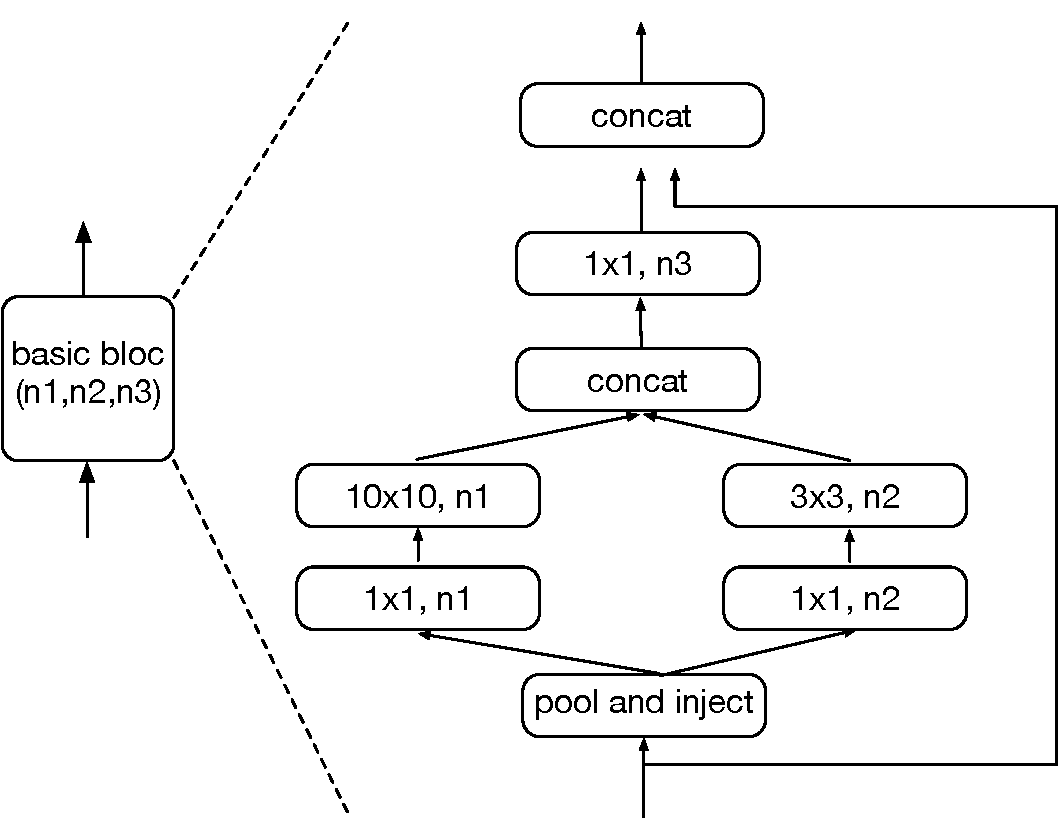
\includegraphics[scale=0.3]{basic_layer}
\caption{Basic Block, or a building block of the environment model's architecture}
\end{figure}

Recall that the state returned by the OpenAI Gym API is just an RGB image, and due to normalization 
described in the Game Environment section, there are only five distinct kinds of pixels: border pixels (black),
background pixels (brown), ball pixels (white), player pixels (green), and opponent pixels (orange).
Therefore, the each pixel in a given state is first mapped to a corresponding index (1 - 5). Then, the action
taken by the model-free agent is converted to a one-hot representation, and concatenated to the
state data. This encodes all state and action information that the environment model needs to begin training.

Next, the input data is sent through a series of convolutional layers, consisting of higher level logical units
called ``basic blocks", as described in the paper. The first layer of a basic block is \emph{pool-and-inject},
which applies a maxpool and concatenates the result to the input. The result is then passed through
two parallel convolutional layers, which are concatenated again for the basic block's final output.

After the basic block units, there is an additional convolutional layer and fully-connected layer for the
state and reward predictions.



\subsection{I2A}

I2A combines the knowledge learned by the models from the previous two steps. Like the model-free A2C, I2A learns a policy, but it also incorporates information from the environment model.

\section{Results}

Here we discuss some results obtained from running components of the I2A network.

\subsection{Model-free agent}

***DRAFT***
A2C was very difficult to train for our current task
Network converges to a suicide strategy, both for pong and for qbert

Average loss is increasing even though the average time discounted rewards is also increasing
The network tends to converge into a losing strategy that has very low critic loss and quickly abandons accidental discoveries of high reward strategies.
***DRAFT***


\begin{figure}[h]
\centering
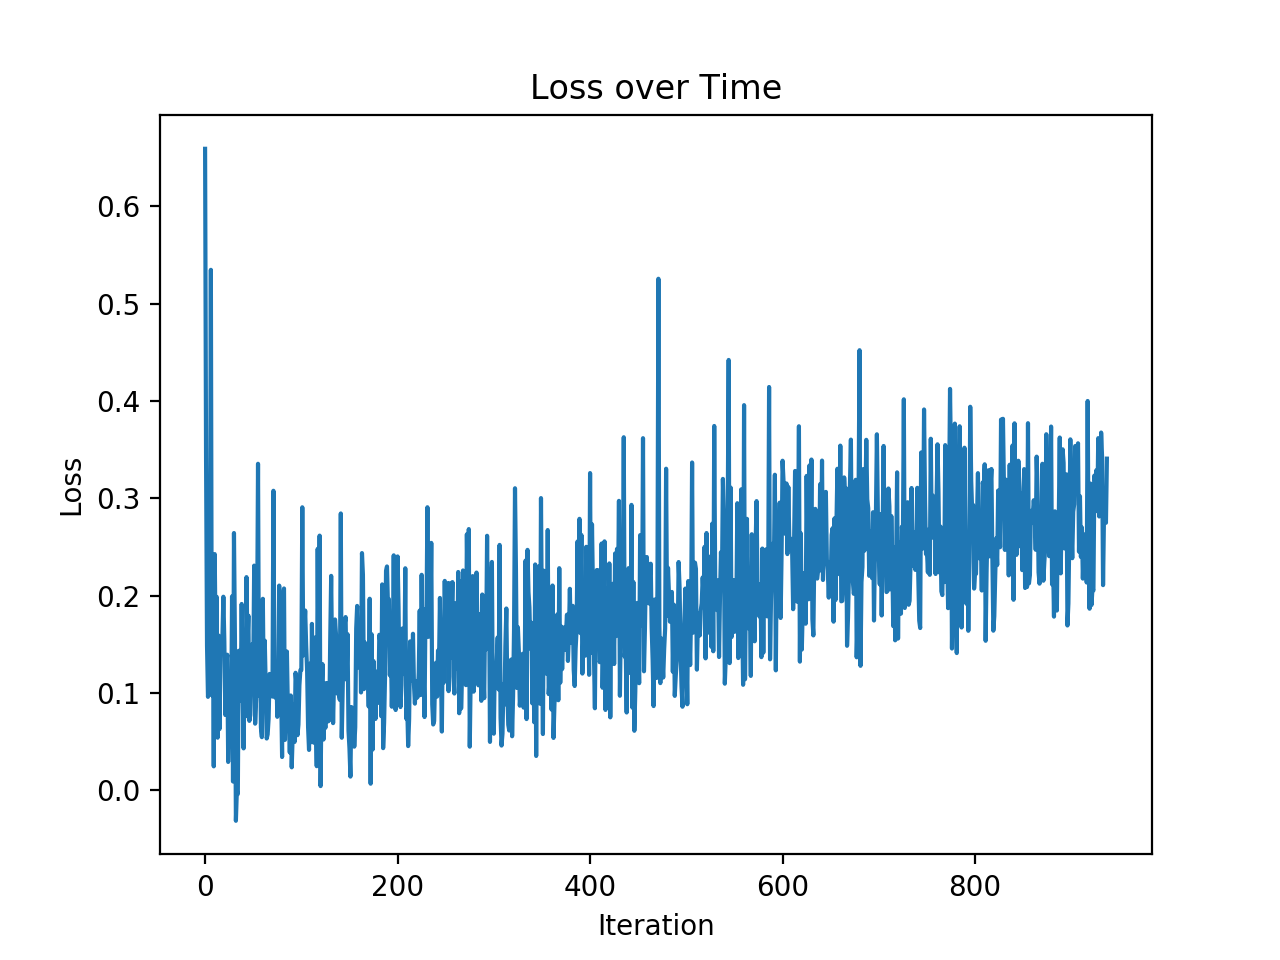
\includegraphics[scale=0.4]{losses}
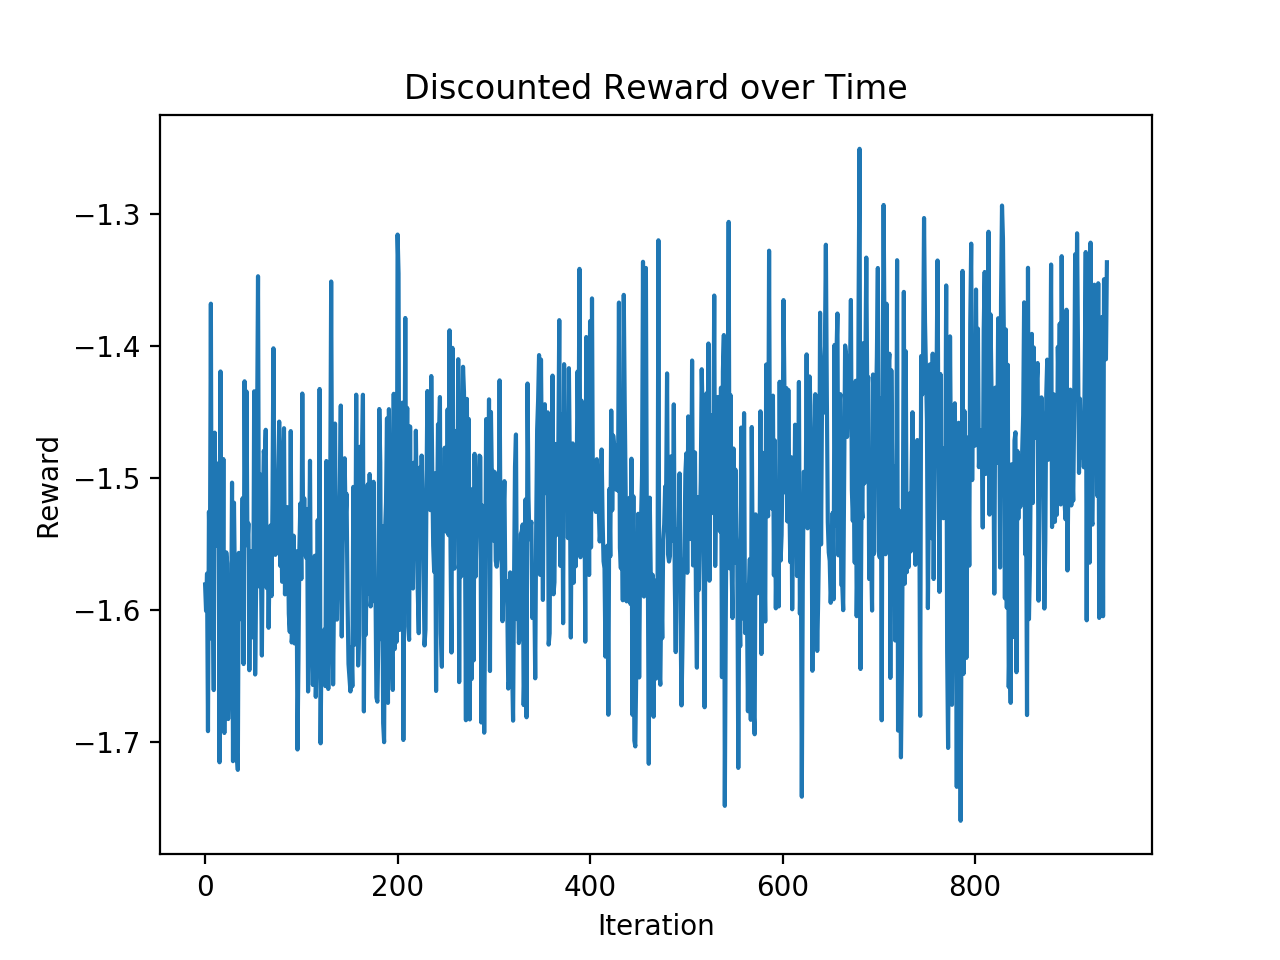
\includegraphics[scale=0.4]{rewards}
\caption{Loss and discounted reward while training the model-free agent.}
\label{plots}
\end{figure}

\subsection{Imagination}

The environment model had moderate success at learning to predict the RGB image of a next state. Typically, when looking at frames
that the model ``imagines", one sees a pattern where the model first learns shape, then learns colors. For example, the model is very quick to learn the border and background boundaries in just a few iterations, even though in the imagined image the background may be green or the border white. It is slower to learn the player, opponent, and ball pixels, though they do eventually appear after several dozen steps of training the environment.

See Figure \ref{imagination} for examples produced by the imagination core. In the figure on the left, only the player is visible, while on the right, some pixels of the opponent are visible. The ball is also visible, though it is more difficult to see, and is not in the correct color, since the model has not yet learned the ball's color.

\begin{figure}[h]
\centering
\begin{subfigure}[b]{.2\textwidth}
  \centering
  \includegraphics[scale=0.5]{player}
  \caption{Player appears}
  \label{fig:player}
\end{subfigure} 
\begin{subfigure}[b]{.2\textwidth}
  \centering
  \includegraphics[scale=0.5]{opponent}
  \caption{Opponent appears}
  \label{fig:opponent}
\end{subfigure} \hfill
\caption{Sample imagined images. The model is quick to learn the background pixels, but takes longer to learn the player, opponent, and ball pixels.}
\label{imagination}
\end{figure}

\section{Discussion}

In this section, we discuss the issues encountered when studying I2A and implementing an architecture for Pong, along with potential solutions that could be implemented in future work.

\subsection{Model-free agent}
***DRAFT***
Model-free agent is an integral part of the whole I2A architecture as it not only is one of the two primary decision pathways alongside the aggregated rollouts, but it is also used while training the environment model and the rollout encoder.

Part of the reason is the decision to use A2C instead of other model free networks like A3C and DQN

A2C is not a good network for a problem like Pong:

	https://eccv18-vlease.github.io/static/papers/drl-video-game.pdf

	Rewards are not immediate

	There are very many states that are similar to the network and yet only a very small subset of these states have rewards, so there is a high critic loss attached to actions that return rewards, meaning the network avoids repeating strategies that were successful. On top of this, state values get harder to learn as the network plays better, since a bad agent consistently gets negative rewards with low variance, while variance of the expected reward increases as the agent gets better and better.

Many approaches were tried to alleviate these problems

	One of the first things was to add an entropy loss to the loss function which is  -entropy_factor* (actProbs*log(actProbs))

	Entropy incentivizes exploration instead of converging to a [1,0,0] probability configuration. 
	While entropy helped, it hampered the network’s ability to precisely adjust the paddle’s position, losing points even when the paddle is mostly in the right position.

	Another problem was that policies that are overall better can perform badly given the arbitrariness in the outcome and how rare the rewards are.
	This results in good strategies being abandoned quickly 

	Batches of 8 games were played before each update to reduce this effect. Larger batches would help even further, but the size of VRAM of the cloud computing instance used did not allow more games to be used in training at once. A better way to alleviate this problem may be to use A3C which has many worker processes that each play individual games, which would mean frequent updates to the network as well as many games with similar policies to get an average effectiveness of the policy. 

	Another approach that was tried was to alter the loss contribution of the critic, but that prevents the critic from learning state values and is thus slows down network convergence even further.

***DRAFT***

\subsection{Environment}
As previously stated, the environment model used for Pong is a modification of the one used by MiniPacman. Between the environments of MiniPacman and Sokoban, we believe that the former is better suited to Pong since its pool-and-inject layer considers global information about the environment. However, in a more thorough study of I2A applied to Pong, one should further consider how the environment can be best tuned specifically to Pong. It is possible there is a significantly different environment architecture that is performs better than what is used in this work.

Another critical difference between Pong and MiniPacman is the difference in size between the RGB images of the two games. MiniPacman is quite small, even by Atari 2600's standard, and is represented as a 15 x 19 grid world. By contrast, Atari's Pong has a 210 x 160 pixel representation, which is roughly two orders of magnitude larger than MiniPacman. Therefore, it is possible that using larger or deeper networks than the one used in MiniPacman would result in much better performance. Alternatively, one could design a Pong game from scratch that uses substantially fewer pixels, since the game has very low complexity. Unfortunately, the original paper did not provide any specifications on the hardware used for training their models.

\subsection{Future Work}


\bibliographystyle{plain}{
\bibliography{report}
}

\end{document}
